% Page settings
\documentclass[notitlepage,12pt]{article}
\usepackage{fancyvrb, verbatim, listings}                                  % Various for inserting/hosting code
\usepackage{setspace}                                                      % Space between lines (customisable)
\usepackage[margin=2.54cm]{geometry}                                       % Set margins (standard is 2.54cm)
\usepackage[UKenglish,cleanlook]{isodate}                                  % Set default date and date display
\usepackage{fancyhdr} \pagestyle{fancy}                                    % Line the top of the page
\usepackage[activate={true,nocompatibility},final,tracking=true,kerning=true,spacing=true,factor=1100,stretch=10,shrink=10]{microtype}
\microtypecontext{spacing=nonfrench}                                       % Change font and minor spacings to look nicer
\setlength{\parskip}{0.5\baselineskip}                                     % Set default paragraph behaviour: skip a line
%\setlength{\parindent}{0pt}                                                % Set default paragraph behaviour: no indent
%% Packages to use:
% Tables + figures
\usepackage{graphicx}                                                      % control over the import of graphics
\usepackage[table,dvipsnames]{xcolor}                                      % Define tables (with colour control)
\usepackage{float}                                                         % Control over graphics + tables float
\usepackage[justify]{ragged2e}                                             % control over text alignment
\usepackage{booktabs}                                                      % caption graphics + tables (with name in bold)
\usepackage[labelfont=bf]{caption} 
\usepackage{subcaption}
\usepackage[shortlabels]{enumitem}                                         % Customisable lists
% caption graphics + tables (with name in bold)
\usepackage{tikz}
\usetikzlibrary{shapes,decorations,decorations.pathreplacing,arrows,calc,arrows.meta,fit,positioning}
\tikzset{
    auto,node distance =1 cm and 1 cm,semithick,
    state/.style ={ellipse, draw, minimum width = 0.7 cm},
    point/.style = {circle, draw, inner sep=0.04cm,fill,node contents={}},
    bidirected/.style={Latex-Latex,dashed},
    el/.style = {inner sep=2pt, align=left, sloped}
}
%\usepackage{pgfplots} \pgfplotsset{compat=1.16}                            % Automatic graphing, read https://www.overleaf.com/learn/latex/pgfplots_package for examples
% Maths + numbers
\usepackage{mathtools}                                                     % Various maths functions
\usepackage{amssymb}                                                       % Various maths functions
\usepackage{amsmath}                                                       % Various maths functions
\usepackage{dsfont}                                                        % Various maths functions
\usepackage{centernot}                                                     % center \not usage
\usepackage{siunitx} \sisetup{round-mode=places, round-precision=3}        % Formalise use of units and numbers among text
\usepackage{amsthm}                                                        % NEvrionemtn for theorems.
\newtheorem{theorem}{Theorem}                                              % Define theorem environment.
\newtheorem{assumption}{Assumption}                                        % Define assumptions environment ahead of theorems.
\newtheorem{definition}{Definition}                                        % Define definitions environment ahead of theorems.
\DeclareMathOperator{\eps}{\varepsilon}                                    % epsilon short hand shortcut
\DeclareMathOperator{\st}{\text{ s.t. }}                                   % "such that" short hand shortcut
\DeclareMathOperator{\then}{\text{ then }}                                 % "then" in equation shortcut
\DeclareMathOperator{\ifeq}{\text{ if }}                                   % "if" in equation shortcut
\DeclareMathOperator{\oreq}{\text{ or }}                                   % "or" in equation shortcut
\DeclareMathOperator{\andeq}{\text{ and }}                                 % "and" in equation shortcut
\DeclareMathOperator{\all}{,\; \text{ for }}                                    % all (with spacing) in equation shortcut
\DeclareMathOperator{\N}{\mathbb{N}}                                       % N, natural number, shortcut
\DeclareMathOperator{\R}{\mathbb{R}}                                       % R, real number, shortcut
\DeclareMathOperator{\Ll}{\mathcal{L}}                                     % L, Lagrangian, shortcut
\renewcommand{\vec}[1]{\boldsymbol{\mathit{#1}}}                           % vector notation shortcut
\newcommand{\mat}[1]{\boldsymbol{\mathit{#1}}}                             % matrix notation shortcut
\DeclarePairedDelimiter\abs{\lvert}{\rvert}                                % absolute value notation shortcut
\DeclarePairedDelimiter\norm{\lVert}{\rVert}                               % norm notation shortcut
\newcommand{\Prob}[1]{\Pr\left( #1 \right)}                         % SHortcut for probability notation
\newcommand{\Probgiven}[2]{\Pr\left( #1 \, \middle\vert \, #2 \right)} % SHortcut for probability notation, given
\newcommand{\E}[2][]{\mathbb{E}_{#1} \left[ #2 \right]}                    % Expectation (with optional subscript) shortcut
\newcommand{\Egiven}[3][]{\mathbb{E}_{#1} \left[ #2 \, \middle\vert \, #3 \right]} % Expectation given (with optional subscript) shortcut
\newcommand{\Var}[2][]{\text{Var}_{#1} \left( #2 \right)}                  % Variation (with optional subscript) shortcut
\newcommand{\Cov}[1]{\text{Cov} \left( #1 \right)}                         % Covariance (with optional subscript) shortcut
\newcommand{\median}[1]{\text{median} \left( #1 \right)}                   % Median (with optional subscript) shortcut
\newcommand{\indicator}[1]{\mathds{1}\left\{ #1 \right\}}                  % SHortcut for indicator function
\newcommand{\diff}[2][]{\frac{d#1}{d#2}}                                   % SHortcut for differential fraction as a function
\newcommand{\partialdiff}[2][]{\frac{\partial#1}{\partial#2}}              % SHortcut for partial differential fraction as a function
\newcommand{\converge}[1]{\xrightarrow{ #1 \to\infty}}                     % SHortcut for convergence arrow
\renewcommand{\hat}[1]{\widehat{#1}}                                       % Default estimator notation is widehat
\renewcommand{\bar}[1]{\overline{#1}}                                      % Make over bar look nicer
\renewcommand{\tilde}[1]{\widetilde{#1}}                                   % Make over tilde look better
\newcommand{\indep}{\, \raisebox{0.05em}{\rotatebox[origin=c]{90}{$\models$}} \,}% Statistical independence symbol.
\definecolor{ao(english)}{rgb}{0.0, 0.5, 0.0}                              % Define dark green colour 
% Citations
\usepackage{natbib} %[longnamesfirst]                                  % Citation package, see https://en.wikibooks.org/wiki/LaTeX/Bibliography_Management#Natbib
\usepackage[backref=page]{hyperref}                                        % Allow for links across the text, with colour options
\hypersetup{colorlinks=true, linkcolor=blue, citecolor=blue, filecolor=magenta, urlcolor=blue}
\def\sectionautorefname~#1\null{Section~#1\null}                           % Fix autoref for sections
\def\subsectionautorefname~#1\null{Subsection~#1\null}                     % Fix autoref for subsections
\def\subsubsectionautorefname~#1\null{Subsubsection~#1\null}               % Fix autoref for subsubsections
\def\equationautorefname~#1\null{Equation~(#1)\null}                       % Fix autoref for equations
% IMPORTANT: follow style guide here https://github.com/Wookai/paper-tips-and-tricks
\usepackage{epigraph}                                                      % Package for quoting from elsewhere.


%%%%%%%%%%%%%%%%%%%%%%%%%%%%%%%%%%%%%%%%
%% Title page
% Author
\author{Senan Hogan-Hennessy\thanks{
    % This work has been supported by research grants from the Centre for the Study of Inequality and Economics Department, Cornell University.
    For helpful comments I thank
    Neil Cholli,
    Luk\'a\u{s} Laff\'ers,
    Yiqi Liu,
    Douglas Miller,
    Zhuan Pei,
    and
    Brenda Prallon.
    % I thank seminar participants at Cornell University (2023, 2024), Norway School of Economics (2024) for helpful discussion.
    Any comments or suggestions may be sent to me at \href{mailto:seh325@cornell.edu}{\nolinkurl{seh325@cornell.edu}}.
    %, or raised as an issue on the Github project.
    } \\
    \vspace{0.1cm}
    Economics Department, Cornell University\footnote{
        Address: Uris Hall \#447, Economics Department, Cornell University NY 14853 USA.
    }
}
% Title
\title{Causal Mediation in Natural Experiments}
\date{This version: \today \\ \vspace{0.25cm}
    \textbf{\textit{Aspirational Abstract, please do not circulate.}}
    %\textbf{\textit{Work-in-Progress, please do not circulate.}}
    %\href{https://github.com/shoganhennessy/mr-education}{Newest version available here.}
    \vspace{-0.5cm}
}
\rhead{\today}
\lhead{Causal Mediation in Natural Experiments.}
% Begin
\begin{document}
\clearpage
\maketitle
\thispagestyle{empty}
% Abstract
\begin{abstract}
    \noindent
Natural experiments are a cornerstone of applied economics, providing settings for estimating causal effects with a compelling argument for treatment ignorability.
Economists are often interested in understanding the mechanisms through which causal treatment effects operate, and Causal Mediation (CM) methods aid this by estimating how much of the treatment effect operates through a proposed mediator.
The most popular CM approach relies on assumptions which are unrealistic in natural experiment settings: assuming the mediator is conditionally ignorable --- in addition to the ignorability argument for the initial treatment.
This paper shows that this approach leads to biased inference, solving for explicit bias terms when the mediator is not ignorable.
Using the case of a Roy model for a mediator, I show that individuals' selection based on expected gains and costs is inconsistent with mediator ignorability without implausible behavioural assumptions, and that bias terms are large in practice.
I show a control function approach, which overcomes these hurdles if monotonicity holds, using cost of mediator take-up as an instrument.
Simulations confirm that this method corrects for persistent bias in conventional CM estimates, and performs comparably to a selection-on-observables approach when the structural assumptions do not hold.
% I illustrate the approach by estimating the proportion of the causal effect of genes associated with education that operates via a direct genetic channel versus indirectly through extended schooling.
% Finally, I provide an implementation of this method in the \textit{R} package \textit{mediate-controlfun}, offering an accessible tool for robust mediation analysis in natural experiment settings.
This approach gives applied researchers a practical method to estimate CM effects when they can only establish a credible argument for randomisation of the initial treatment, as is common in natural experiments.

\vspace{0.5cm}
\noindent
\textbf{Keywords:}
Direct/indirect effects, quasi-experiment, selection, control function.

\vspace{0.1cm}
\noindent
\textbf{JEL Codes:}
D31, D91, I24, J24, Z00.

\end{abstract}

%%%%%%%%%%%%%%%%%%%%%%%%%%%%%%%%%%%%%%%%%
%% Starting the paper
\newpage
\setcounter{page}{1}
\doublespacing
% Introduction section
\noindent
%\section{Introduction}
%\label{sec:intro}
% \textbf{The introduction formula \url{https://blogs.ubc.ca/khead/research/research-advice/formula}.}
%\textbf{Hook:}
Economists use natural experiments to credibly answer social questions, when an experiment was infeasible.
For example, does access to health insurance causally improve health and well-being \citep{finkelstein2008oregon}?
Natural experiments are settings which answer these questions, but give little indication of how these effects came about.
Causal Mediation (CM) aims to estimate the mechanisms behind causal effects, by estimating how much of the treatment effect operates through a proposed mediator.
For example, do causal gains from access to health insurance come mostly from starting to utilise healthcare more often, or are there other direct effects?
This study of mechanisms behind causal effects broadens the economic understanding of social settings studied with natural experiments.
This paper shows that the conventional approach to estimating CM effects is inappropriate in a natural experiment setting, provides a theoretical framework for how bias operates, and develops an approach to correctly estimate CM effects under alternative assumptions.
These methods contrast the current practice in applied economics of providing suggestive evidence of mechanisms, which does not identify or quantify causal effects.

% Paragraph here: how do applied economists currently do it?
% Summarise my work with the Finkelstein+ data.

%\textbf{Question:}
This paper starts by considering conventional CM methods in a natural experiment setting.
Conventional CM methods rely on assuming the initial treatment, and the subsequent mediator, are both ignorable \citep{imai2010identification}.
In a natural experiment setting, however, this may not hold true; 
winners of the Oregon Health Insurance Experiment wait-list lottery randomly received access to health insurance, but then chose of their own free will how often to use healthcare.
Here, conventional CM estimates for the average direct and indirect effects will be contaminated by bias terms, from not accounting for selection-into-healthcare.
Indeed, it is unlikely conventional CM estimates in any natural experiment will lead to credible causal effects, unless researchers use another natural experiment to isolate random variation in the mediator (at the same time as using one for the initial treatment).

I consider an alternative approach to estimating CM effects, adjusting for unobserved selection-into-mediator via identifying the marginal treatment effect of the mediator.
This solves the identification problem with structural assumptions for selection-into-mediator --- mediator monotonicity and selection based on benefits --- and requires a valid cost instrument for mediator take-up.
While these assumptions are strong, they are plausible in many applied settings.
Mediator monotonicity aligns with conventional theories for selection-into-treatment, and is accepted widely in many applications using an instrumental variables research design.
Selection based on costs and benefits is central to economic theory, and is the dominant concern for judging empirical designs that identify causal effects.
Access to valid instrumental variation is a strong condition, though is important to avoid further modelling assumptions; the most compelling example is using variation in mediator take-up costs as an instrument.
This approach is not perfect in every setting: the structural assumptions are strong, and are tailored to selection-into-mediator concerns pertinent to economic applications.
Indeed, this approach provides no safe harbour for estimating CM effects if these structural assumptions do not hold true.

%Paragraph on the results of the Oregon experiment.

%\textbf{Antecedents:}
Assuming the mediator is quasi-randomly assigned conveniently ignores selection by assuming either (1) people na\"ively made decisions to take or refuse a mediator, or (2) a researcher controlled for everything relevant to this decision.
This assumption might be reasonable when studying single-celled organisms in a laboratory --- their ``decisions'' are simple and mechanical.
Social scientists, however, study humans who make complex choices based on costs, benefits, and preferences --- which are only partially observed by researchers, at best.
Assuming a mediator is ignorable in social science contexts is often unrealistic.
In practice, the main setting where mediator ignorability becomes credible is when researchers find another natural experiment affecting the mediator --- a rare occurrence given how difficult it is to find one source of random variation for a treatment, let alone another independent source for a mediator, at the same time.

The applied economics literature has been hesitant to use explicit CM methods, instead providing suggestive evidence for mechanisms,\footnote{
    See \cite{blackwell2024assumption} for an overview of this approach, from the empirical politics literature.
} sometimes accompanied by a practice of controlling for a proposed mediator.
Neither of these approaches have a causal interpretation.
A new strand of the econometric literature has developed estimators for explicit CM analyses under a variety of strategies.
These include overlapping quasi-experimental research designs \citep{deuchert2019direct,frolich2017direct}, functional form restrictions \citep{heckman2015econometric,heckman2013understanding}, partial identification \citep{flores2009identification}, or a hypothesis test of full mediation through observed channels \citep{kwon2024testing} --- see \cite{huber2019review} for an overview.\footnote{
    An alternative method to estimate CM effects is ensuring treatment and mediator ignorability holds by a running two randomised controlled trials for both treatment and mediator, at the same time.
    This set-up has been considered in the literature previously, in theory \citep{imai2013experimental} and in practice \citep{ludwig2011mechanism}.
}
The new literature has arisen in implicit acknowledgement that suggestive evidence of mechanisms, or a conventional approach to CM, can lead to biased inference and needs alternative methods for credible inference.

%\textbf{Value-added:}
I develop a framework showing exactly how selection bias contaminates CM estimates when mediator choices are driven by unobserved gains --- settings where none of the natural experiment research designs in the previously cited papers apply (i.e., the mediator is not ignorable).
This provides a rigorous warning to applied economists against uncritically applying conventional CM methods to investigate mechanisms in natural experiments --- as is common in the applied fields of epidemiology, psychology, and medicine.
Selection based on costs and benefits, as in the \cite{roy1951some} model, is at odds with assuming a mediator is randomly assigned in an observational setting, so I import methods grounded in labour economic theory to solve the identification problem.

Identifying CM effects via the marginal treatment effect of the mediator requires mediator take-up respond only positively to the initial treatment (monotonicity), which implies mediator selection follows a selection model.
Second, it assumes that mediator take-up is motivated by mediator benefits.
Last, it requires a valid instrument for mediator take-up, to avoid relying on parametric assumptions on unobserved selection.
This approach to identifying CM effects imports insights from the instrumental variables literature, connecting the influential \cite{imai2010identification} approach to CM with the economics literature on selection-into-treatment and marginal treatment effects \citep{vytlacil2002independence,heckman2004using,heckman2005structural,florens2008identification,kline2019heckits}.
%\footnote{
%    Indeed, this paper does not invent control function methods, instead noting their applicability in this setting.
%    See \cite{wooldridge2015control,imbens2007nonadditive} for general overviews of the approach.
%}
\cite{frolich2017direct} have previously explored identification of CM effects with a control function in the context of two instruments (one each for treatment and mediator) and a continuous mediator.
This paper considers the marginal treatment effect of a binary mediator, with a correspondingly different identification analysis and resulting estimation strategies.

%\textbf{Road-map:}
This paper proceeds as follows.
\autoref{sec:lottery} describes the dominant approach in economics for studying mechanisms behind treatment effects, illustrating with data from the Oregon Health Insurance Experiment.
% and surveys economic research.
\autoref{sec:mediation} introduces the formal framework for CM, and develops expressions for bias in CM estimates in natural experiments.
\autoref{sec:applied} describes this bias in applied settings with (1) a regression framework, (2) a setting with selection based on costs and benefits.
\autoref{sec:selectionmodel} purges bias from CM estimates by identifying CM effects via the marginal treatment effect of the mediator, with a control function adjustment.
\autoref{sec:controlfun} demonstrates how to estimate CM effects with this approach, with either parametric or semi-parametric methods, giving supporting simulation evidence.
\autoref{sec:oregon} returns to the Oregon Health Insurance Experiment, providing credible estimates of access to health insurance effects on self-reported health and well-being mediated through healthcare usage.
\autoref{sec:conclusion} concludes.

% Conceptual Framework
\section{Direct and Indirect Effects}
\label{sec:concepts}
Causal mediation decomposes causal effects into two channels, through a mediator (indirect effect) and through all other paths (direct effect).

%\textbf{To add: Why do we even want these effects?}

To develop notation for direct and indirect effects, write $Z_i$ for an exogenous binary variable, $D_i$ an intermediary outcome, and $Y_i$ an outcome for individuals $i = 1, \hdots, n$.
The outcomes are a sum of their potential outcomes:
\begin{align*}
    D_i &= Z_i       D_i(1)
        + (1 - Z_i) D_i(0),  \\
    Y_i &= Z_i       Y_i(1, D_i(1))
        + (1 - Z_i) Y_i(0, D_i(0))
\end{align*}
$Z_i$ affects outcome $Y_i$ directly, and indirectly via the $D_i(Z_i)$ channel, with no reverse causality.
The framework is general to any (conditionally) randomly assigned $Z_i$, selected mediator $D_i$, and outcome $Y_i$.
For the analysis in \autoref{sec:data}, $Z_i$ is the Ed PGI, $D_i$ a measure of education year, and $Y_i$ (log) later-life earnings.
Note that     $Z_i, D_i$ are continuous measures in HRS Data, but this section focuses on binary $Z_i, D_i = 0,1$ to simplify the causal framework.\footnote{
    Continuous analogues of the following are extensions of the binary case, and will be included in work to follow.
    %\autoref{appendix:continuous} relates the causal framework to continuous $Z_i,D_i$, which has little conceptual differences.
}
\autoref{fig:scm-model} visualises the design, where the direction arrows denote the causal direction (and no reverse causality).

\begin{figure}[h!]
    \centering
    \singlespacing
    \caption{Structural Causal Model for Direct and Indirect Effects of Genetics and Education.}
    \label{fig:scm-model}
    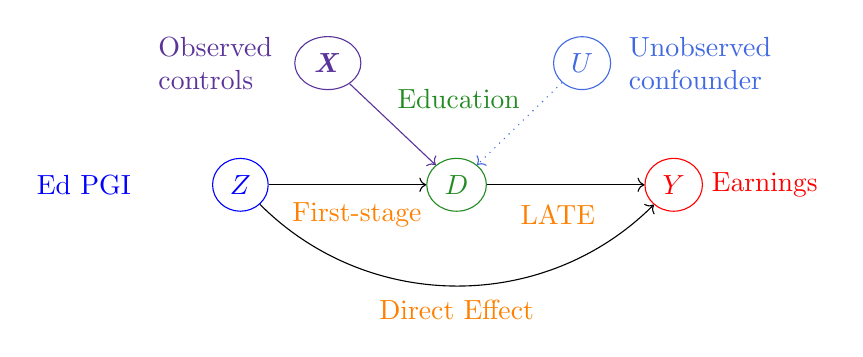
\begin{tikzpicture}
        \node[state,ForestGreen] (treatment) at (0,0) {$D$};
        \node[state,blue] (instrument) [left=2cm of treatment] {$Z$};
        \node[state,red] (outcome) [right=2cm of treatment] {$Y$};
        \path[->] (instrument) edge (treatment);
        \path[->] (treatment) edge (outcome);
        % Label the nodes with econ examples
        \node[text width=2cm, color=blue] [left=0.1cm of instrument] {Ed PGI};
        \node[text width=0.1cm, color=red] [right=-0.01cm of outcome] {Earnings};
        \node[text width=1.5cm, color=ForestGreen] [above=0.5cm of treatment] {Education};
        % Add in direct effects.
        \path[->] (instrument) edge[bend right=45] (outcome);
        % Label the causal effects
        \node[text height=1cm, color=orange] [left=0.5cm of outcome] {LATE};
        \node[text height=1cm, color=orange] [right=0.175cm of instrument] {First-stage};
        \node[text height=1cm, color=orange] [below=0.25cm of treatment] {Direct Effect};
        % Add in the confounders
        \node[state,RoyalPurple] (confounderX) [above left=1.5cm of treatment] {$\vec{X}$};
        \path[->,RoyalPurple] (confounderX) edge (treatment);
        \node[text width=1.5cm, color=RoyalPurple] [left=0.1cm of confounderX] {Observed controls};
        \node[state,RoyalBlue] (confounderU) [above right=1.5cm of treatment] {$U$};
        \path[->,dotted,color=RoyalBlue] (confounderU) edge (treatment);
        \node[text width=2.5cm, color=RoyalBlue] [right=0.1cm of confounderU] {Unobserved confounder};
    \end{tikzpicture}
    \justify
    \footnotesize
    \textbf{Note}:
    This figures shows the structural causal model for decomposing the direct and indirect effects of genetics and education attainment.
\end{figure}

Assuming that Ed PGI $Z_i$ is randomly assigned (or conditionally so, see \autoref{sec:data-genescore}), then there are only two average effects which are identified.
The first-stage effect refers to the effect of the Ed PGI on education, $Z \to D$.
\[ \Egiven{D_i}{Z_i = 1} - \Egiven{D_i}{Z_i = 0}
    = \E{D_i(1) - D_i(0)} \]
It common in the economics literature to assume that $Z$ influences $D$ in at most one direction, $\Prob{D_i(1) \geq D_i(0)} = 1$ --- monotonicity \citep{imbens1994identification}.
I assume monotonicity (and its conditional variant) holds through-out, as it brings the mediation notation closer to the IV literature from labour economics.\footnote{
    Monotonicity has other beneficial implications in this setting, as shown in \autoref{sec:selection-model}.
} 

The reduced-form effect refers to the effect of the Ed PGI on earnings, $Z \to Y$, and is also known as the intent-to-treat effect in experimental settings, or total effect in causal mediation literature.
\[ \Egiven{Y_i}{Z_i = 1} - \Egiven{Y_i}{Z_i = 0}
    = \E{Y_i(1, D_i(1)) - Y_i(0, D_i(0))} \]

On the other hand, mediation aims to decompose the reduced form effect of $Z \to Y$ into two separate pathways: indirectly through $D$, and directly absent $D$.
\begin{align*}
    \text{Indirect Effect, } D(Z) \to Y: \;\;\;&
        \E{Y_i(Z_i, D_i(1)) - Y_i(Z_i, D_i(0))} \\
    \text{Direct Effect, } Z \to Y: \;\;\;&
        \E{Y_i(1, D_i(Z_i)) - Y_i(0, D_i(Z_i))}
\end{align*}
These effects are not separately identified without further assumptions.

\subsection{Causal Mediation Estimates}
The conventional approach to estimating direct and indirect effects assumes both $Z_i$ and $D_i$ are conditionally ignorable.
\begin{definition}
    \label{dfn:seq-ign}
    Sequential Ignorability \citep{imai2010identification}.
    \begin{align}
        \label{eqn:seq-ign-Z}
        Z_i \indep  D_i(z), Y_i(z', d) \;\; &| \;\; \vec X_i,
            &\textnormal{ for } z, z', d = 0, 1 \\
        \label{eqn:seq-ign-D}
        D_i \indep  Y_i(z', d) \;\; &| \;\; \vec X_i, Z_i = z', 
            &\textnormal{ for } z', d = 0, 1
    \end{align}
\end{definition}
If \ref{dfn:seq-ign}\eqref{eqn:seq-ign-Z} and \ref{dfn:seq-ign}\eqref{eqn:seq-ign-D} hold, then the direct and indirect effects are identified by two-stage mean differences, after conditioning on $\vec X_i$:\footnote{
    \cite{imai2010identification} show a general identification statement; I show identification in terms of two-stage regression, which is more familiar in economics.
    This reasoning is in line with G-computation reasoning \citep{robins1986g};
    \autoref{appendix:identification} states the \cite{imai2010identification} identification result, and then develops the two-stage regression notation which holds as a consequence of sequential ignorability.
}

\makebox[\textwidth]{\parbox{1.25\textwidth}{
\[ \E[D_i, \vec X_i]{
    \underbrace{\Egiven{Y_i}{Z_i = 1, D_i, \vec X_i} - \Egiven{Y_i}{Z_i = 0, D_i, \vec X_i}}_{\text{Second-stage regression, $Y_i$ on $Z_i$ holding $D_i$ constant}}}
    = \underbrace{\E{Y_i(1, D_i(Z_i)) - Y_i(0, D_i(Z_i))}}_{\text{Average Direct effect}} \]
\[ \E[Z_i, \vec X_i]{ \underbrace{\Big(
    \Egiven{D_i}{Z_i = 1, \vec X_i} - \Egiven{D_i}{Z_i = 0, \vec X_i} \Big)}_{\text{First-stage regression, $D_i$ on $Z_i$}}
    \times \underbrace{\Big(
    \Egiven{Y_i}{Z_i, D_i = 1, \vec X_i} - \Egiven{Y_i}{Z_i, D_i = 0, \vec X_i} \Big)}_{\text{Second-stage regression, $Y_i$ on $D_i$ holding $Z_i$ constant}} } \]
\[ = \underbrace{\E{Y_i(Z_i, D_i(1)) - Y_i(Z_i, D_i(0))}}_{\text{Average Indirect effect}} \]
}}

These estimands are typically estimated with linear models \citep{imai2010identification}:
\begin{align*}
    D_i &= \phi + \pi Z_i
        + \vec \psi_1' \vec X_i+ \eta_i \\
    Y_i &= \alpha + \beta D_i + \gamma Z_i + \delta Z_i D_i
        + \vec \psi_2' \vec X_i + \varepsilon_i
\end{align*}
And so the direct and indirect effects are composed from OLS estimates,
$\hat \gamma + \hat\delta \E{D_i}$ for the direct effect and
$\hat\pi \left(\hat \beta + \E{Z_i} \hat \delta \right)$ for the indirect effect.
While this is the most common approach in the applied literature, I do not focus on the linear formulation of this problem as it assumes homogenous treatment effects and linear confounding.
These assumptions are unnecessary to my analysis; it suffices to note that heterogeneous treatment effects and non-linear confounding would bias OLS estimates of direct and indirect effects in the same manner that is well documented elsewhere (see e.g., \citealt{angrist1998estimating,sloczynski2022interpreting}).
I focus on fundamental problems that plague causal mediation methods in practice, regardless of estimation method.
As such, I focus my work on non-parametric identification, and employ semi- and non-parametric estimation methods in my empirical analysis  whenever possible to avoid these problems.

\subsection{Selection Bias in Causal Mediation Estimates}
Mediation methods are the main method that researchers then answer the following question: how did $Z$ lead to a causal effect on $Y$, and through which channels?
In observational work this may include a natural experiment that quasi-randomly assigns $Z_i$ to individuals, regardless of their preferences or selection patterns --- i.e., justifying assumption \ref{dfn:seq-ign}\eqref{eqn:seq-ign-Z}.
Rarely does observational research employ an additional, overlapping identification design for $D_i$ as part of the analysis, and instead they employ mediation methods by assuming this $D_i$ is ignorable given observed covariates $\vec X_i$.\footnote{
    \cite{imai2013experimental} call attention to the need for a separate research design to isolate causal effects of $D_i$ in randomised controlled trials; \autoref{appendix:mediation-review} overviews literature, finding many papers that employ mediation methods with a research design for $Z_i$, but not for $D_i$.
}
This approach leads to biased estimates, and contaminates inference regarding direct and indirect effects (in the same manner as \citealt{heckman1998characterizing}).

\begin{theorem}
    \label{thm:selection-bias}
    Absent an identification strategy for the mediator, causal mediation estimates are at risk of selection bias.
    Suppose \ref{dfn:seq-ign}\eqref{eqn:seq-ign-Z} holds, but \ref{dfn:seq-ign}\eqref{eqn:seq-ign-D} does not.
    Then causal mediation estimates are contaminated by selection bias terms, and group differences terms.
\end{theorem}
\begin{proof}
    See \autoref{appendix:selection-bias} for the extended proof.
\end{proof}
Below I present the relevant selection bias and group difference terms, omitting the conditional on $\vec X_i$ notation for brevity.
These selection bias terms would be equal to zero if the mediator was conditional ignorable \eqref{eqn:seq-ign-D}, but do not necessarily average to zero if not.

For the average direct effect: CM estimate $=$ ADE $+$ selection bias $+$ group differences.
\vspace{-0.5cm}
\begin{align*}
    & \mathbb E_{D_i} \Big[
        \Egiven{Y_i}{Z_i = 1, D_i} - \Egiven{Y_i}{Z_i = 0, D_i} \Big] \\
    & = \E{Y_i(1, D_i(Z_i)) - Y_i(0, D_i(Z_i))} \\
    & \;\;\;\; + \mathbb E_{D_i} \Big[
        \Egiven{Y_i(0, D_i(Z_i))}{D_i(1) = d} 
        - \Egiven{Y_i(0, D_i(Z_i))}{D_i(0) = d} \Big] \\
    & \;\;\;\; + \E[D_i ]{
        \Big(1 - \Prob{D_i(1) = d} \Big)
        \left( \begin{aligned}
            &\Egiven{Y_i(1, D_i(Z_i)) - Y_i(0, D_i(Z_i))}{D_i(1) = d} \\ 
            &  - \Egiven{Y_i(1, D_i(Z_i)) - Y_i(0, D_i(Z_i))}{D_i(0) = 1- d}
            \end{aligned} \right) }
\end{align*}

For the average indirect effect: CM estimate $=$ AIE $+$ selection bias $+$ group differences.
\vspace{-0.5cm}
\begin{align*}
    &\E[Z_i]{
        \Big( \Egiven{D_i}{Z_i = 1} - \Egiven{D_i}{Z_i = 0} \Big) \times
        \Big( \Egiven{Y_i}{Z_i, D_i = 1} - \Egiven{Y_i}{Z_i, D_i = 0} \Big) } \\
    & = \E{Y_i(Z_i, D_i(1)) - Y_i(Z_i, D_i(0))} \\
    & \;\;\;\; + \Prob{D_i(1) = 1, D_i(0) = 0} \Big(
        \Egiven{Y_i(Z_i, 0)}{D_i = 1} - \Egiven{Y_i(Z_i, 0)}{D_i = 0} \Big) \\
    & \;\;\;\; + \Prob{D_i(1) = 1, D_i(0) = 0} \times \\
    & \;\;\;\; \;\; \left[ \begin{aligned}
        &\Big( 1 - \Prob{D_i=1} \Big)
        \left( \begin{aligned}
            &\Egiven{Y_i(Z_i, 1) - Y_i(Z_i, 0)}{D_i = 1} \\ 
            &  - \Egiven{Y_i(Z_i, 1) - Y_i(Z_i, 0)}{D_i = 0}
        \end{aligned} \right) \\
        &+ \left( \frac{1 - \Prob{D_i(1) = 1, D_i(0) = 0} }{
            \Prob{D_i(1) = 1, D_i(0) = 0}} \right)
        \left( \begin{aligned}
            &\Egiven{Y_i(Z_i, 1) - Y_i(Z_i, 0)}{D_i(1) = 0 \text{ or } D_i(0)=1} \\ 
            &  - \E{Y_i(Z_i, 1) - Y_i(Z_i, 0)}
        \end{aligned} \right)
    \end{aligned} \right]
\end{align*}

The selection bias terms come from systematic differences between the treated and untreated groups, differences not fully unexplained by $\vec X_i$.
The group differences represent the fact that a matching estimator gives an average effect on the treated group and, when selection-on-observables does not hold, this is systematically different from the average effect \citep{heckman1998characterizing}.\footnote{
    The selection-on-observables approach could, instead, focus on the average effect on treated populations (as do \citealt{keele2015identifying}).
    This runs into a problem of comparisons: CM estimates would give average effects on different treated groups.
    The CM estimate for the ADE on treated gives the ADE local to the $Z_i = 1$ treated group, while the AIE estimate gives the AIE local to the $D_i = 1$ group.
    In this way, these ADE and AIE on treated terms are not comparable to each other, so I focus on the true average terms.
}
The group differences term is longer for the average indirect effect estimate, because the indirect effect is comprised from the effect of $D_i$ local to $Z_i$ compliers; a matching estimator gets the average effect on treated, and the longer term adjusts for differences with the complier average effect.

% Econometric Framework, mediation under selection
\section{Direct and Indirect Effects Under Selection}
\label{sec:metrics}
This section connects causal mediation, without assuming the mediator is randomly assigned (i.e., under selection), with classic labour economics models for selection into treatment.

\subsection{Selection Model Representation}
\label{sec:selection-model}
The IV literature assumes a first-stage monotonicity condition, where randomised $Z_i$ influences mediator $D_i$ in at most one direction.
\begin{definition}
    \label{dfn:firststage-monotonicity}
    First-stage Monotonicity \citep{imbens1994identification}.
    \begin{equation}
        \label{eqn:firststage-monotonicity}
        \Prob{ D_i(1) \geq D_i(0)} = 1    
    \end{equation}
\end{definition}

Assuming \ref{dfn:firststage-monotonicity}\eqref{eqn:firststage-monotonicity}
in a mediation setting opens mediation to the wide literature on IV and selection models for identification in the presence of selection. 
\begin{theorem}
    \label{thm:selection-model}
    Under monotonicity, mediator $D_i$ can be represented by a selection model. \\
    Suppose \ref{dfn:firststage-monotonicity}\eqref{eqn:firststage-monotonicity} holds, then there is a function $\mu(.)$ and random variable $U_i$ such that $D_i$ takes the following form.
    \[ D_i(z) = \indicator{ \mu(z) \geq U_i}, \;\; \forall z = 0,1 \]
\end{theorem}
\begin{proof}
    Special case of the \cite{vytlacil2002independence} equivalence result; see \autoref{appendix:selection-model}.
\end{proof}

\autoref{thm:selection-model} is a powerful result: it says that at the cost of assuming monotonicity (as is done in the IV literature), then selection into $D_i$ takes a latent index form, and opens up identification in a mediation context to the wide literature on identifying treatment effects in selection models.

\subsection{A Regression Framework for Direct and Indirect Effects}
Inference for direct and direct effects can be written in a regression framework, showing how correlation between the error term and the mediator persistently biases estimates.
And thus, selection models can be used to adjust for unobserved confounding.

To motivate a regression framework with unobserved confounding, write $Y_i(Z, D)$ as a sum of observed factors $Z_i, \vec X_i$ and unobserved factors, (following the notation of \citealt{heckman2005structural}).
First, define the following unobserved error terms
\[ U_{0,i} = Y_i(Z_i, 0) - \Egiven{Y_i(Z_i, 0)}{\vec X},\;\;\;\;
U_{1,i} = Y_i(Z_i, 1) - \Egiven{Y_i(Z_i, 1)}{\vec X} \]

Then observed data take the following representation, which characterises direct effects, indirect effects, and the selection problem (see \autoref{appendix:regression-model} for all definitions).
\begin{align*}
    D_i &= \phi_i + \pi_i Z_i + \eta_i  \\
    Y_i &= \alpha_i + \beta_i D_i + \gamma_i Z_i + \delta_i Z_i D_i
    + \underbrace{U_{0,i} + D_i \left( U_{1,i} - U_{0,i} \right)}_{
        \text{Correlated error term.}}
\end{align*}
And the average direct and indirect effects are given by the following
\begin{align*}
    \E{Y_i(Z_i, D_i(1)) - Y_i(Z_i, D_i(0))}
        &= \E{\left( \beta_i +  Z_i \delta_i \right) \times \pi_i}, \\
    \E{Y_i(1, D_i(Z_i)) - Y_i(0, D_i(Z_i))}
        &= \E{\gamma_i + \delta_i D_i}.
\end{align*}

By assumption $Z_i \indep Y_i(.,.), D_i(.)$, so that the regression only gives unbiased estimates if $D_i$ is also conditionally random: $D_i \indep U_{0, i} - U_{1, i} \; | \; \vec X_i$.
If not, then the regression estimates (without adjusting for the contaminated bias term) suffer from omitted variables bias.

\subsection{Selection into Education}
In the education context, point identifying direct and indirect effects requires the \textit{researcher controls for all sources of selection-into-education}.

While this assumption may hold true in two-way randomised experiments (e.g., in a laboratory or two-way RCT), it is unlikely to hold in the case of quasi-experimental variation in $Z$, or when modelling education as a mediator --- absent a separate identification strategy for education $D$.
To expand this point in an econometric selection-into-treatment framework, suppose selection follows a Roy model, where individual $i$ weighs the costs and benefits of completing education.
\[ D_i(Z_i) = \indicator{
    \underbrace{C_i(Z_i)}_{\text{Costs}}
    \leq
    \underbrace{Y_i(Z_i, 1) - Y_i(Z_i, 0)}_{\text{Gains}}} \]
Education choice $D_i(z)$ is clearly related to $Y_i(z, d)$ in this model, so let's see what the equation looks like in terms of sequential ignorability.
As above, decompose costs into observed and unobserved factors.
\[ C_i(Z_i) = \mu_{C}(Z_i; \vec X_i) + U_{C,i} \]

And so we can write the first-stage selection equation in full.
\begin{align*}
    D_i(z) &= \indicator{
        \underbrace{U_{C, i} + U_{0, i} - U_{1, i}}_{\text{Unobserved}}
        \leq
        \underbrace{
            \mu_1(z; \vec X_i) - \mu_0(z; \vec X_i)- \mu_C(z; \vec X_i)}_{\text{Observed}}}
\end{align*}
Sequential ignorability, where $Y_i(z, d) \indep D_i(z') \; | \; \vec X_i$, would then require that $\Egiven{U_{0, i} - U_{1, i}}{D_i} = 0$.
In the Roy model above, this would assume every single contribution for returns to education is contained in $\vec X_i$; if there are any unobserved sources by which people have systematically different returns to education, then they would select into education based on this, and bias na\"ive mediation estimates.
This is unlikely to hold true, unless there is another identification strategy for $D_i$ --- in addition to the one used for $Z_i$.

\subsection{Estimating Direct and Indirect Effects}

Quasi-experimental work does not take the assumption of ``selection-on-observables'' at face value without an explicit research design \citep{angrist2009mostly} or modelling approach to address this issue.

A classical approach to modelling this issue, is a selection model approach \citep{heckman1974shadow,heckman1979sample}.
The approach assume $U_0, U_1$ follow a known distribution (e.g, bivariate normal), and estimates the regression via maximum likelihood.
Alternatively, a control function approach estimates the system in two stages, avoiding (some) distributional assumptions if an instrument is used, at the cost of efficiency.
In the following, I estimate direct and indirect effects first by OLS (assuming sequential ignorability), and then via both variants of the sample selection models, to compare estimates.
Future work will consider estimates by using an alternative instrument for education, in the framework of \cite{frolich2017direct} to avoid the modelling assumptions inherent to sample selection models.

% Discussion Section
\section{Discussion and Future Work}
\label{sec:discussion}

This project aims to achieve two main goals:
first, to test the claims that genetics (specifically Ed PGI) is associated with labour market outcomes independently, and secondly to connect the mediation literature to classical labour economic methods for adjusting for selection bias.
Adjusting conventional mediation methods via a structural selection model for education reduces estimates for the direct channel in the genetic association from $~50\%$ to $~0\%$.
These results bring into question previous claims, in the context of Ed PGI, that genetics affect outcomes independently of education.

This work so far has focused on genetic association, and not causal effects, because the HRS data have no clear research design for random variation in Ed PGI.
This means that the above estimates are only correlational because the EA Score is heritable, and not randomized.
However, there is opportunity to analyse random genetic variation, thanks to Mendelian independent assortment.
If a father has an Ed PGI of $X$ and a mother $Y$, then genetic mixing at conception means their child is expected to have an EA Score of $\frac{X+Y}{2}$.
Thanks to genetic mixing, their child may have EA Score above or below the expected value, as they randomly inherited more/fewer genes in the EA Score from the parent with a higher score (a.k.a. random Mendelian segregation, \citealt{young2018relatedness}).
The HRS has no data on parental genetic information, so the estimates above did not control for parents' scores and are thus not causal \citep{young2022mendelian}.
In-progress work is expanding on the above, using UK Biobank data on genetic data after controlling for parents genes, expanding these results from genetic associations to genetic effects.

Secondly, this project has so far connected causal mediation to classical approaches to selection into treatment, using a Roy model as a key structural example for which selection models can overcome selection bias in mediation analyses.
However, an explicit research design for years of education (in addition to Ed PGI) is necessary for realistic estimates --- in the sense of a causally identified analysis \citep{angrist2009mostly}.
An overlapping instrument for years of education is necessary to compare to the results of classical sample selection models.

% Conclusion Section
%%%%%%%%%%%%%%%%%%%%%%%%%%%%%%%%%%%%%%%%%%
%% Conclusion section
\section{Summary and Concluding Remarks}
\label{sec:conclusion}

This paper studies the returns to higher education, using IV methods from the epidemiology literature and adjustments from the causal mediation literature to tackle violations of the exclusion restriction.
First, I derive identification of the average mechanism effect under a selection-on-observables type assumption, and partial identification when unobserved selection confounding.
I apply these methods to a sample of retirement age Americans in the years 1990--2021, using genetic information to instrument for higher education, estimating that higher education leads to roughly 40\% higher earnings (point estimates), or between 8--44\% higher earnings (partial bounds).
Additionally, women had significantly higher returns to higher education over this time period.

The methods here provide alternatives to assuming the exclusion restriction in empirical applications of IV models, so can be useful in sensitivity analyses for any application of IV methods.
Mendelian randomisation is a particularly useful application of IV methods, though the exclusion restriction is particularly problematic in practice.
The approach allows researchers to use MR to study effects of both health conditions and behaviours with significant selection-into-treatment concerns, such as higher education.


% Bibliography
\singlespacing
\bibliographystyle{agsm}
\bibliography{sections/08-bibliography.bib}
%\bibliography{sections/08-bibliography-doi.bib}
% Appendix
\newpage
%%%%%%%%%%%%%%%%%%%%%%%%%%%%%%%%%%%%%%%%%
%% Appendix section
% Set-up the section.
%\newpage
\appendix
\setcounter{table}{0}
\renewcommand{\thetable}{A\arabic{table}}
\setcounter{figure}{0}
\renewcommand{\thefigure}{A\arabic{figure}}

% Start appendix
\section{Appendix}
\label{appendix}
This project used computational tools which are fully open-source.
%As such, all code and data involved in this project are available at this project's Github repository, available at \url{https://github.com/shoganhennessy/state-faculty-composition}.
%They may be used for replication, or as the basis for further work, as needed.
Any comments or suggestions may be sent to me at \href{mailto:seh325@cornell.edu}{\nolinkurl{seh325@cornell.edu}}, or raised as an issue on the Github project.

A number of statistical packages, for the R language \citep{R2023}, made the empirical analysis for this paper possible.
\begin{itemize}
    \item \textit{Tidyverse} \citep{tidyverse} collected tools for data analysis in the R language.
    \item \textit{DoubleML} \citep{DoubleML2020} implemented doubly robust methods used in the empirical analysis. 
    \item \textit{GRF} \citep{athey2019generalized,grf} compiled forest computational tools for the R language.
    \item \textit{Stargazer} \citep{stargazer} provided methods to efficiently convert empirical results into presentable output in \LaTeX.
\end{itemize}

\subsection{Identification in Causal Mediation}
\label{appendix:identification}
\citet[Theorem~1]{imai2010identification} states that the direct and indirect effects are identified under sequential ignorability, at each level of $Z_i = 0,1$.
For $z' = 0,1$: \\
\makebox[\textwidth]{\parbox{1.25\textwidth}{
\begin{align*}
    \E{ Y_i(1, D_i(z')) - Y_i(0, D_i(z'))}
    &= \int \int 
    \Big( \Egiven{ Y_i }{Z_i = 1, D_i, \vec X_i}
        - \Egiven{ Y_i }{Z_i = 0, D_i, \vec X_i} \Big)
            dF_{D_i \, | \, Z_i = z', \vec X_i} dF_{\vec X_i}, \\
    \E{ Y_i(z', D_i(1)) - Y_i(z', D_i(0))}
    &= \int \int \Egiven{ Y_i }{Z_i = z', D_i, \vec X_i}
    \Big( dF_{D_i \, | \, Z_i = 1, \vec X_i}
        - dF_{D_i \, | \, Z_i = 0, \vec X_i} \Big) dF_{\vec X_i}.
\end{align*}
}}
I focus on the averages, which are identified by consequence of the above.
\begin{align*}
    \E{ Y_i(1, D_i(Z_i)) - Y_i(0, D_i(Z_i))}
    &= \E[Z_i]{\Egiven{ Y_i(1, D_i(z')) - Y_i(0, D_i(z'))}{Z_i = z'}} \\
    \E{ Y_i(Z_i, D_i(1)) - Y_i(Z_i, D_i(0))}
    & = \E[Z_i]{\Egiven{ Y_i(z', D_i(1)) - Y_i(z', D_i(0))}{Z_i = z'}}
\end{align*}
My estimand for the average direct effect is a simple rearrangement of the above.
The estimand for the average indirect effect relies on a different sequence, relying on (1) sequential ignorability, (2) conditional monotonicity.
These give (1) identification of, and equivalence between, LADE conditional on $\vec X_i$ and ADE conditional on $\vec X_i$, (2) identification of the complier score.

\begin{align*}
    & \Egiven{ Y_i(Z_i, D_i(1)) - Y_i(Z_i, D_i(0))}{\vec X_i} \\
    & = \Probgiven{D_i(1) = 1, D_i(0) = 0}{\vec X_i}
        \Egiven{ Y_i(Z_i, 1) - Y_i(Z_i, 0)}{D_i(1) = 1, D_i(0) = 0, \vec X_i} \\
    & = \Probgiven{D_i(1) = 1, D_i(0) = 0}{\vec X_i}
        \Egiven{ Y_i(Z_i, 1) - Y_i(Z_i, 0)}{\vec X_i} \\
    & = \Big( \Egiven{D_i}{Z_i = 1, \vec X_i} - \Egiven{D_i}{Z_i = 0, \vec X_i}
        \Big) \; \Egiven{ Y_i(Z_i, 1) - Y_i(Z_i, 0)}{\vec X_i} \\
    & = \Big( \Egiven{D_i}{Z_i = 1, \vec X_i} - \Egiven{D_i}{Z_i = 0, \vec X_i}
        \Big)
        \Big( \Egiven{Y_i}{Z_i, D_i = 1, \vec X_i}
            - \Egiven{Y_i}{Z_i, D_i = 0, \vec X_i} \Big)
\end{align*}
Monotonicity is not technically required for the above.
Breaking monotonicity would not change the identification of any of the above; it would be the same except replacing the complier score with a complier or defier score, $\Probgiven{D_i(1) \neq D_i(0)}{\vec X_i} = \Egiven{D_i}{Z_i = 1, \vec X_i} - \Egiven{D_i}{Z_i = 0, \vec X_i}$.

\subsection{Continuous Average Causal Responses}
\label{appendix:continuous}
Section here relating the approach to the average causal response function (see e.g., Angrist Imbens JASA 1996, Andrew Bacon for DiD 2023).

\subsection{Previous Literature}
\label{appendix:mediation-review}

Create a table in this section that surveys previous research which employs mediation methods while having a clear causal design for $Z_i$, but not $D_i$.

\begin{tabular}{l l l l l}
    Paper & Field & Research Design for $Z_i$ & Research Design for $D_i$ & Selection bias? \\ \hline
    Paper name 1.    
\end{tabular}

\subsection{Bias in Mediation Estimates}
\label{appendix:mediation-bias}
Suppose that $Z_i$ is ignorable conditional on $\vec X_i$, but $D_i$ is not.

\subsubsection{Bias in Direct Effect Estimates}
To show that the conventional approach to mediation gives an estimate for the ADE with selection and non-complier bias, start with the components of the conventional estimands.
This proof starts with the relevant expectations, conditional on a specific value of $\vec X_i$.
For each $d' =0, 1$.
\begin{align*}
    \Egiven{Y_i}{Z_i = 1, D_i = d', \vec X_i}
    =& \Egiven{Y_i(1, D_i(Z_i))}{D_i(1) = d', \vec X_i}, \\
    \Egiven{Y_i}{Z_i = 0, D_i = d', \vec X_i}
    =& \Egiven{Y_i(0, D_i(Z_i))}{D_i(0) = d', \vec X_i}
\end{align*}
And so
\begin{align*}
    &  \Egiven{Y_i}{Z_i = 1, D_i = d', \vec X_i}
    - \Egiven{Y_i}{Z_i = 0, D_i = d', \vec X_i} \\
    =& \Egiven{Y_i(1, D_i(Z_i))}{D_i(1) = d', \vec X_i}
    - \Egiven{Y_i(0, D_i(Z_i))}{D_i(0) = d', \vec X_i} \\
    =& \Egiven{Y_i(1, D_i(Z_i)) - Y_i(0, D_i(Z_i))}{D_i(1) = d', \vec X_i} \\
    &+ \Egiven{Y_i(0, D_i(Z_i))}{D_i(1) = d', \vec X_i}
        - \Egiven{Y_i(0, D_i(Z_i))}{D_i(0) = d', \vec X_i} 
\end{align*}
The final term is a sum of the ADE, conditional on $D_i(1) = d'$, and a selection bias term --- difference in baseline terms between the (partially overlapping) groups for whom $D_i(1) = d'$ and $D_i(0) = d'$.

To reach the final term, note the following.
\begin{align*}
    &\Egiven{Y_i(1, D_i(Z_i)) - Y_i(0, D_i(Z_i))}{\vec X_i} \\    
    =& \Egiven{Y_i(1, D_i(Z_i)) - Y_i(0, D_i(Z_i))}{D_i(1) = d', \vec X_i} \\
    &+ \Big(1 - \Probgiven{D_i(1) = d'}{\vec X_i}\Big)
    \left( \begin{aligned}
        &\Egiven{Y_i(1, D_i(Z_i)) - Y_i(0, D_i(Z_i))}{D_i(1) = d', \vec X_i} \\ 
        & - \Egiven{Y_i(1, D_i(Z_i)) - Y_i(0, D_i(Z_i))}{D_i(1) = 1 - d', \vec X_i}
    \end{aligned} \right) 
\end{align*}
The second term is a difference term between the average and the average for relevant complier groups.

Collect everything together, as follows.
\begin{align*}
    &  \Egiven{Y_i}{Z_i = 1, D_i = d', \vec X_i}
    - \Egiven{Y_i}{Z_i = 0, D_i = d', \vec X_i} \\
    =& \underbrace{
        \Egiven{Y_i(1, D_i(Z_i)) - Y_i(0, D_i(Z_i))}{\vec X_i}}_{
            \text{ADE, conditional on }\vec X_i} \\
    &+ \underbrace{
        \Egiven{Y_i(0, D_i(Z_i))}{D_i(1) = d', \vec X_i}
            - \Egiven{Y_i(0, D_i(Z_i))}{D_i(0) = d', \vec X_i}}_{
                \text{Selection bias}} \\
    &+ \underbrace{\Big(1 - \Probgiven{D_i(1) = d'}{\vec X_i}\Big)
    \left( \begin{aligned}
        &\Egiven{Y_i(1, D_i(Z_i)) - Y_i(0, D_i(Z_i))}{D_i(1) = d', \vec X_i} \\ 
        & - \Egiven{Y_i(1, D_i(Z_i)) - Y_i(0, D_i(Z_i))}{D_i(1) = 1 - d', \vec X_i}
    \end{aligned} \right)}_{
        \text{Non-complier bias}}
\end{align*}
The proof is achieved by applying the expectation across $D_i = d'$, and $\vec X_i$.

\subsubsection{Bias in Indirect Effect Estimates}
To show that the conventional approach to mediation gives an estimate for the AIE with selection and non-complier bias, start with the definition of the ADE --- the direct effect among compliers times the size of the complier group.

This proof starts with the relevant expectations, conditional on a specific value of $\vec X_i$.
\begin{align*}
    &\Egiven{ Y_i(Z_i, D_i(1)) - Y_i(Z_i, D_i(0))}{\vec X_i} \\
    =& \Probgiven{D_i(1) = 1, D_i(0) = 0}{\vec X_i}
        \Egiven{ Y_i(Z_i, 1) - Y_i(Z_i, 0)}{D_i(1) = 1, D_i(0) = 0, \vec X_i}
\end{align*}
When $D_i$ is not ignorable, the bias comes from estimating the second term,\\ $\Egiven{ Y_i(Z_i, 1) - Y_i(Z_i, 0)}{D_i(1) = 1, D_i(0) = 0, \vec X_i}$.

For each $z' =0, 1$.
\begin{align*}
    \Egiven{Y_i}{Z_i = z', D_i = 1, \vec X_i}
    =& \Egiven{Y_i(z', 1)}{D_i = 1, \vec X_i}, \\
    \Egiven{Y_i}{Z_i = z', D_i = 0, \vec X_i}
    =& \Egiven{Y_i(z', 0)}{D_i = 0, \vec X_i}
\end{align*}
So compose the CM estimand, as follows.
\begin{align*}
    & \Egiven{Y_i}{Z_i = z', D_i = 1, \vec X_i}
    - \Egiven{Y_i}{Z_i = z', D_i = 0, \vec X_i} \\
    =& \Egiven{Y_i(z', 1)}{D_i = 1, \vec X_i}
        - \Egiven{Y_i(z', 0)}{D_i = 0, \vec X_i} \\
    =& \Egiven{Y_i(z', 1) - Y_i(z', 0)}{D_i = 1, \vec X_i}
    + \Egiven{Y_i(z', 0)}{D_i = 1, \vec X_i} - \Egiven{Y_i(z', 0)}{D_i = 0, \vec X_i}
\end{align*}
The final term is a sum of the AIE, among the treated group $D_i = 1$, and a selection bias term --- difference in baseline terms between the groups $D_i = 1$ and $D_i = 0$.

The AIE is the direct effect among compliers times the size of the complier group, so we need to compensate for the difference between the treated group $D_i = 1$ and complier group $D_i(1)= 1, D_i(0) = 0$.

Start with the difference between treated group's average and overall average.
\begin{align*}
    & \Egiven{Y_i(z', 1) - Y_i(z', 0)}{D_i = 1, \vec X_i} \\
    =& \Egiven{Y_i(z', 1) - Y_i(z', 0)}{\vec X_i} \\
    &+ \Big(1 - \Probgiven{D_i = 1}{\vec X_i} \Big)
    \left( \begin{aligned}
        &\Egiven{Y_i(z', 1) - Y_i(z', 0)}{D_i = 1, \vec X_i} \\ 
        &  - \Egiven{Y_i(z', 1) - Y_i(z', 0)}{D_i = 0, \vec X_i}
    \end{aligned} \right)
\end{align*}
Then the difference between the compliers' average and the overall average.
\begin{align*}
    & \Egiven{ Y_i(z', 1) - Y_i(z', 0)}{D_i(1) = 1, D_i(0) = 0, \vec X_i} \\
    =& \Egiven{Y_i(z', 1) - Y_i(z', 0)}{\vec X_i} \\
    & + \frac{1 - \Probgiven{D_i(1) = 1, D_i(0) = 0}{\vec X_i} }{
        \Probgiven{D_i(1) = 1, D_i(0) = 0}{\vec X_i}}
    \left( \begin{aligned}
        &\Egiven{Y_i(z', 1) - Y_i(z', 0)}{D_i(1) = 0 \text{ or } D_i(0)=1, \vec X_i} \\ 
        &  - \Egiven{Y_i(z', 1) - Y_i(z', 0)}{\vec X_i}
    \end{aligned} \right)
\end{align*}

Collect everything together, as follows.
\begin{align*}
    &  \Egiven{Y_i}{Z_i = z', D_i = 1, \vec X_i}
    - \Egiven{Y_i}{Z_i = z', D_i = 0, \vec X_i} \\
    =& \underbrace{
        \Egiven{Y_i(z', D_i(1)) - Y_i(z', D_i(0))}{\vec X_i}}_{
            \text{AIE, conditional on }\vec X_i, Z_i = z'} \\
    &+ \underbrace{
        \Egiven{Y_i(z', 0)}{D_i = 1, \vec X_i}
            - \Egiven{Y_i(z', 0)}{D_i = 0, \vec X_i}}_{
                \text{Selection bias}} \\
    &+ \underbrace{\left[ \begin{aligned}
        &\Big(1 - \Probgiven{D_i = 1}{\vec X_i} \Big)
        \left( \begin{aligned}
            &\Egiven{Y_i(z', 1) - Y_i(z', 0)}{D_i = 1, \vec X_i} \\ 
            &  - \Egiven{Y_i(z', 1) - Y_i(z', 0)}{D_i = 0, \vec X_i}
        \end{aligned} \right) \\
        &+ \frac{1 - \Probgiven{D_i(1) = 1, D_i(0) = 0}{\vec X_i} }{
            \Probgiven{D_i(1) = 1, D_i(0) = 0}{\vec X_i}} 
        \left( \begin{aligned}
            &\Egiven{Y_i(z', 1) - Y_i(z', 0)}{D_i(1) = 0 \text{ or } D_i(0)=1, \vec X_i} \\ 
            &  - \Egiven{Y_i(z', 1) - Y_i(z', 0)}{\vec X_i}
        \end{aligned} \right)
    \end{aligned} \right] }_{
        \text{Non-complier bias}}
\end{align*}
The proof is finally achieved by multiplying by the complier score, 
$\Probgiven{D_i(1) = 1, D_i(0) = 0}{\vec X_i}$
$= \Egiven{D_i}{Z_i = 1, \vec X_i} - \Egiven{D_i}{Z_i = 0, \vec X_i}$,
then applying the expectation across $Z_i = z'$, and $\vec X_i$.





\subsection{Proof of the Selection Model Representation}
\label{appendix:selection-model}
Write the proof in here, following \cite{vytlacil2002independence} construction in the forward direction.
Note that the notation needs updating for no exclusion restriction.

\subsection{A Regression Framework for Direct and Indirect Effects}
\label{appendix:regression-model}
Put $\mu_{D}(Z; \vec X) = \Egiven{Y_i(Z, D)}{\vec X}$ and $U_{D, i} = Y_i(Z,D) - \mu_D(Z; \vec X)$, so we have the following expressions.
\[ Y_i(Z_i, 0)
        = \mu_{0}(Z_i; \vec X_i) + U_{0,i}, \;\;
    Y_i(Z_i, 1)
        = \mu_{1}(Z_i; \vec X_i) + U_{1,i} \]

$U_{0,i}, U_{1,i}$ are error terms with unknown distributions, mean independent of $Z_i, \vec X_i$ by definition --- but possibly correlated with $D_i$.

$Z_i$ is independent of potential outcomes, so that $U_{0,i}, U_{1,i} \indep Z_i$.
Thus, the first-stage regression of $Z \to Y$ has unbiased estimates.
\begin{align*}
    D_i &= Z_i D_i(1) + (1 - Z_i) D_i(0) \\
        &= D_i(0) +
            Z_i \left[ D_i(1) - D_i(0) \right] \\
        &= \underbrace{\Egiven{D_i(0)}{\vec X_i}        
        }_{\text{Intercept}} +
            \underbrace{Z_i \E{ D_i(1) - D_i(0)}}_{
                \text{Regressor}} \\
            & \;\;\;\; + \underbrace{
                D_i(0) - \Egiven{D_i(0)}{\vec X_i}
                + Z_i \big( D_i(1) - D_i(0) - \Egiven{ D_i(1) - D_i(0)}{\vec X_i}\big)}_{
                \text{Mean-zero independent error term, since }Z_i \indep D_i \; | \; \vec X_i} \\
        &\eqqcolon \phi + \pi Z_i + \varphi(\vec X_i) + \eta_i \\
    \implies \Egiven{D_i}{Z_i, \vec X_i}&=
        \phi + \pi Z_i + \varphi(\vec X_i)
        \text{, and thus unbiased estimates since } Z_i \indep \phi, \eta_i.
\end{align*}

$Z_i$ is also assumed independent of potential outcomes $Y_i(,.,)$, so that $U_{0,i}, U_{1,i} \indep Z_i$.
Thus, the reduced form regression $Z \to Y$ also leads to unbiased estimates.

The same cannot be said of the regression that estimates direct and indirect effects, without further assumptions.
\begin{align*}
    Y_i &= Z_i Y_i(1, D_i(1)) + (1 - Z_i) Y_i(0, D_i(0)) \\
        &= Z_i D_i Y_i(1, 1) \\
        & \;\;\;\; + (1 - Z_i) D_i Y_i(0, 1) \\
        & \;\;\;\; + Z_i (1 - D_i) Y_i(1, 0) \\
        & \;\;\;\; + (1 - Z_i) (1 - D_i) Y_i(0, 0) \\
        &= Y_i(0, 0) \\
        & \;\;\;\; + Z_i \left[Y_i(1, 0) - Y_i(0, 0) \right] \\
        & \;\;\;\; + D_i \left[Y_i(0, 1) - Y_i(0, 0) \right] \\
        & \;\;\;\; + Z_i D_i \left[Y_i(1, 1) - Y_i(1, 0)
            - \left( Y_i(0, 1) - Y_i(0, 0) \right)\right]
\end{align*}
And so $Y_i$ can be written as a regression equation in terms of the observed factors and error terms.
\begin{align*}
    Y_i &= \mu_0(0; \vec X_i) \\
        & \;\;\;\; + D_i \left[\mu_1(0; \vec X_i) - \mu_0(0; \vec X_i) \right] \\
        & \;\;\;\; + Z_i \left[\mu_0(1; \vec X_i) - \mu_0(0; \vec X_i) \right] \\
        & \;\;\;\; + Z_i D_i \left[\mu_1(1; \vec X_i) - \mu_0(1; \vec X_i)
            - \left( \mu_1(0; \vec X_i) - \mu_0(0; \vec X_i) \right)\right] \\
        & \;\;\;\; + U_{0,i} + D_i \left( U_{1,i} - U_{0,i} \right) \\
        &\eqqcolon
            \alpha + \beta D_i + \gamma Z_i + \delta Z_i D_i
            + \zeta(\vec X_i)
            + U_{0,i} + D_i \left( U_{1,i} - U_{0,i} \right)
\end{align*}
With the following definitions:
\begin{itemize}
    \item $\alpha = \E{\mu_0(0; \vec X_i)}$ and $\zeta(\vec X_i) = \mu_0(0; \vec X_i) - \alpha$ are the intercept terms.
    \item $\beta = \mu_1(0; \vec X_i) - \mu_0(0; \vec X_i)$ is the indirect effect under $Z_i = 0$
    \item $\gamma = \mu_0(1; \vec X_i) - \mu_0(0; \vec X_i)$ is the direct effect under $D_i = 0$.
    \item $\gamma = \mu_1(1; \vec X_i) - \mu_0(1; \vec X_i)- \left( \mu_1(0; \vec X_i) - \mu_0(0; \vec X_i) \right)$ is the interaction effect.
    \item $U_{0,i} + D_i \left( U_{1,i} - U_{0,i} \right)$ is the remaining error term.
\end{itemize}
This sequence gives us the resulting regression equation:
\[ \Egiven{Y_i}{Z_i, D_i, \vec X_i} =
    \alpha
    + \beta D_i
    + \gamma Z_i
    + \delta Z_i D_i
    + \zeta(\vec X_i)
    + \Egiven{D_i \left( U_{1,i} - U_{0,i} \right)}{\vec X_i} \]
Taking the conditional expectation, and collecting for the expressions of the direct and indirect effects:\footnote{
    These equations have simpler expressions after assuming constant treatment effects in a linear framework;
    I have avoided this as having compliers, and controlling for observed factors $\vec X_i$ only makes sense in the case of heterogeneous treatment effects.
}
\begin{align*}
    \E{Y_i(Z_i, D_i(1)) - Y_i(Z_i, D_i(0))}
        &= \E{\pi \left( \beta +  Z_i \delta \right)} \\
    \E{Y_i(1, D_i(Z_i)) - Y_i(0, D_i(Z_i))}
        &= \E{\gamma + \delta D_i}
\end{align*}
These terms are conventionally estimated in a simultaneous regression \citep{imai2010identification}.

If sequential ignorability does not hold, then the regression estimates from estimating the mediation equations (without adjusting for the contaminated bias term) suffer from omitted variables bias.

\begin{align*}
    \E[\vec X_i]{\Egiven{Y_i}{Z_i = D_i = 0, \vec X_i}}
        &= \E\alpha + \E{D_i \left( U_{1,i} - U_{0,i} \right)} \\
    \E[\vec X_i]{\Egiven{Y_i}{Z_i = 0, D_i = 1, \vec X_i}
        - \Egiven{Y_i}{Z_i = 0, D_i = 0, \vec X_i}}
        &= \E\beta + \frac{
        \Cov{D_i,\; D_i \left( U_{1,i} - U_{0,i} \right)}}{\Var{D_i}} \\
    \E[\vec X_i]{\Egiven{Y_i}{Z_i = 1, D_i = 0, \vec X_i}
        - \Egiven{Y_i}{Z_i = 0, D_i = 0, \vec X_i}}
        &= \E\gamma + \frac{
        \Cov{Z_i,\; D_i \left( U_{1,i} - U_{0,i} \right)}}{\Var{Z_i}} \\
    \E[\vec X_i]{\begin{aligned}
        &\Egiven{Y_i}{Z_i = 1, D_i = 1, \vec X_i}
            - \Egiven{Y_i}{Z_i = 1, D_i = 0, \vec X_i} \\
            &- \left( \Egiven{Y_i}{Z_i = 0, D_i = 1, \vec X_i}
                - \Egiven{Y_i}{Z_i = 0, D_i = 0, \vec X_i} \right)
        \end{aligned}}
    &= \E\delta + \frac{
        \Cov{Z_i D_i,\; D_i \left( U_{1,i} - U_{0,i} \right)}}{\Var{Z_i D_i}}
\end{align*}
And so the direct and indirect effect estimates are contaminated by these bias terms.

% Senan note: should write CM estimand = \E{\gamma + \delta D_i} + bias, where bias is some Cov term.

\end{document}
